%!TEX root = ../../report.tex
\chapter{Conception and initial analysis} % (fold)
\label{cha:analysis}
The process of sketching a bipedal robot as the presented here implies that the essential variables for the design have to be identified and determined aiming at the most optimal solution possible\footnote{Optimality here is measured in terms of the aimed goals, described in \ref{sec:goals}.}.
The important role of the geometrical and inertial mechanical parameters in locomotion control was first proved by \cite{passive_walking}, and their relevance deserves a careful study.
Hence, the sections in this chapter contain the conceptual presentation of a set of design criteria and the first approaches to the construction of the RuBi prototype arisen from the study of these parameters and the application of these criteria.

%!TEX root= ../../../report.tex

\section{Bipedal locomotion} % (fold)
\label{sec:bipedal_walking_and_running_gaits}
This section contains a superficial comparative study of the characteristics of the motion patterns in human walking and running.
The reason is to help justify in the following chapters the decisions taken during the design towards the generation of these gaits.

Although walking and running motion patterns in humans might resemble each other at first glance, they contain important variations that imply that a robot able to walk at a certain speed is not necessary capable of running at the same speed, or running at all.
The existence of the so-called "flight phase" in running but not in walking cycles is the main difference between them.
This phase comprises the period in which there is no contact between the feet and the ground and causes the main variations in energy and trajectory generation.

\subsection{Walking and running gaits comparison} % (fold)
\label{sub:walk_and_run_comparison}
The differences in both joint kinematics and kinetics between both patterns emerged from the distinction mentioned are studied in \cite{grimmer}, Manuscript I, for a wide range of speeds.
From the cited paper it can be seen that the joint positions for a whole cycle in both walking and running patterns are very similar, specially for hip and knee.
Furthermore, the joint velocity profiles have almost the same shape but differ in the magnitudes, being higher the angular speeds reached for running.
Similar conclusions can be extracted from a quick comparison between the torque and power profiles in a running and walking cycle.
While the shapes of the functions for the three joints are very alike, with the biggest differences for the ankle, the values of the curve are in average smaller for human walking than for running.
As expected, the conclusion is that higher requirements for joint speed, torque and power are expected for running, specially for the knees and the ankles.
Besides, the foot strike and impact forces during the landing phase in both cases change, both in intensity and profile.
% subsection walk_and_run_comparison (end)

% section bipedal_walking_and_running_gaits (end)
%!TEX root = ../../../report.tex

\section{Geometrical dimensions of the frame} % (fold)
\label{sec:dimensions}
The selection of the final dimensions of RuBi corresponds to an iterative process in which power requirements and achieving human-like kinematics have been the main constraints when assessing the size of the robot.
A first approach was taken from \cite{grimmer}, Manuscript I, where normalized values of power required per joint and per kilogram of the structure can be found.
The first iteration targeted a robot of dimensions $m = 1Kg$ and length from the hip joint to the tip toes of $L = 0.6 m$ for a fully stretched leg.
The final parameters from the last iteration can be found in ***%***chapter Results

Once estimated an overall length of the structure, an initial value of the dimensions of each link were decided to be obtained based on the German section of the ISO 7250-2 \cite{iso_measurements} and the DIN 33402-2 \cite{din_measurements1} norms, following the idea of mimicking human-like motion as closely as possible.
These two norms are standard references in industry and were considered a general enough source of information.
Figure \ref{fig:human_measurements} depicts some of the human dimensions extracted from the norms and applied to the design of RuBi.
Their names and values for male between 18-65 year old and in percentile 50 can be found in table \ref{tab:din_proportions}.

\begin{figure}[h]
	\centering
	\begin{subfigure}[b]{0.3\textwidth}
        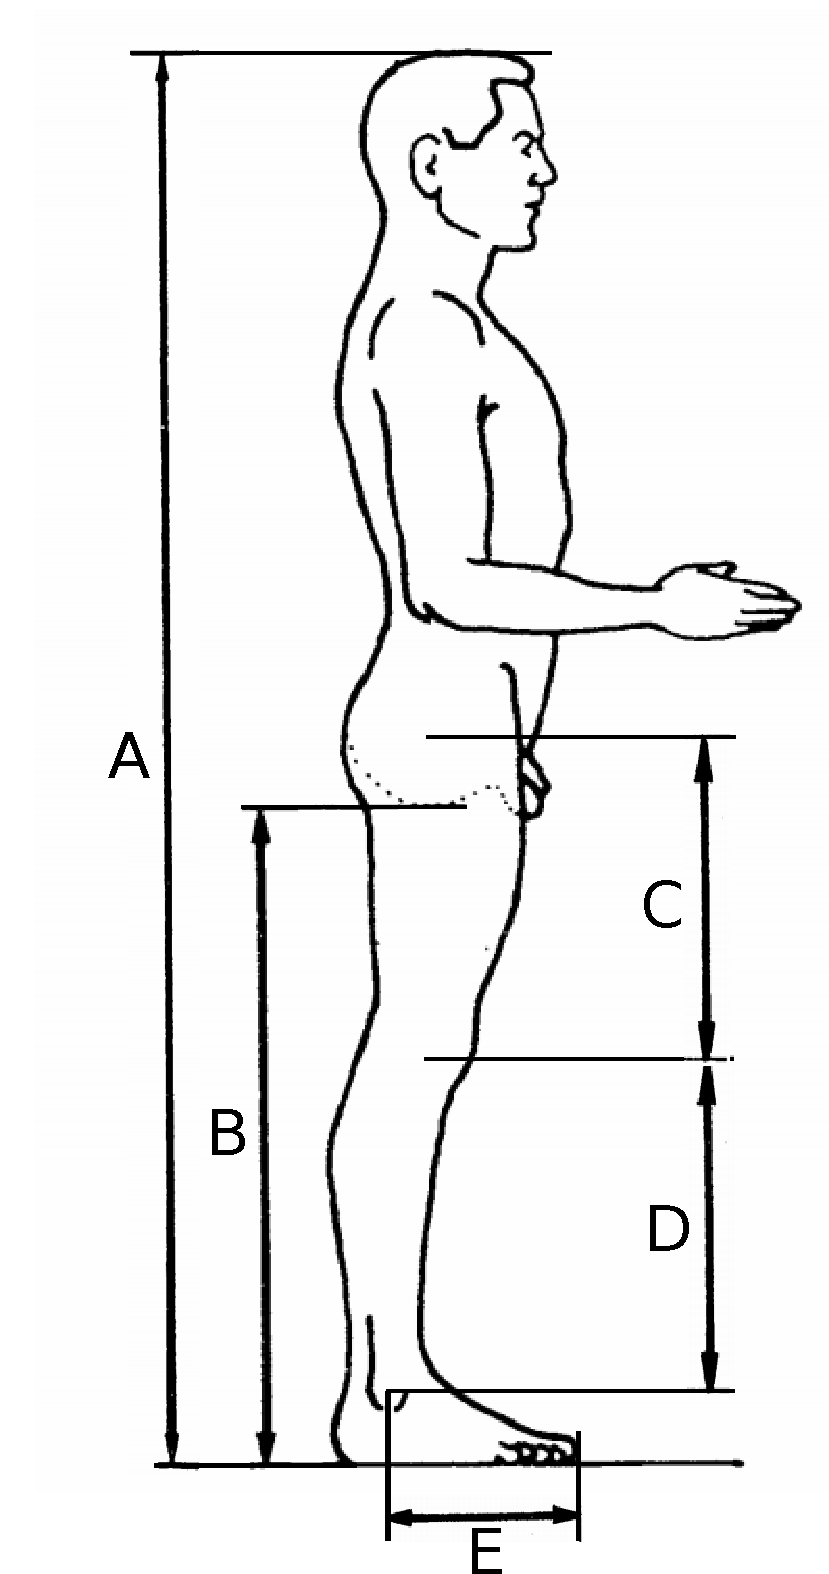
\includegraphics[width=\textwidth]{figures/din_measurements.pdf}
        \caption{Left foot}
        \label{fig:din1}
    \end{subfigure}
    \begin{subfigure}[b]{0.4\textwidth}
        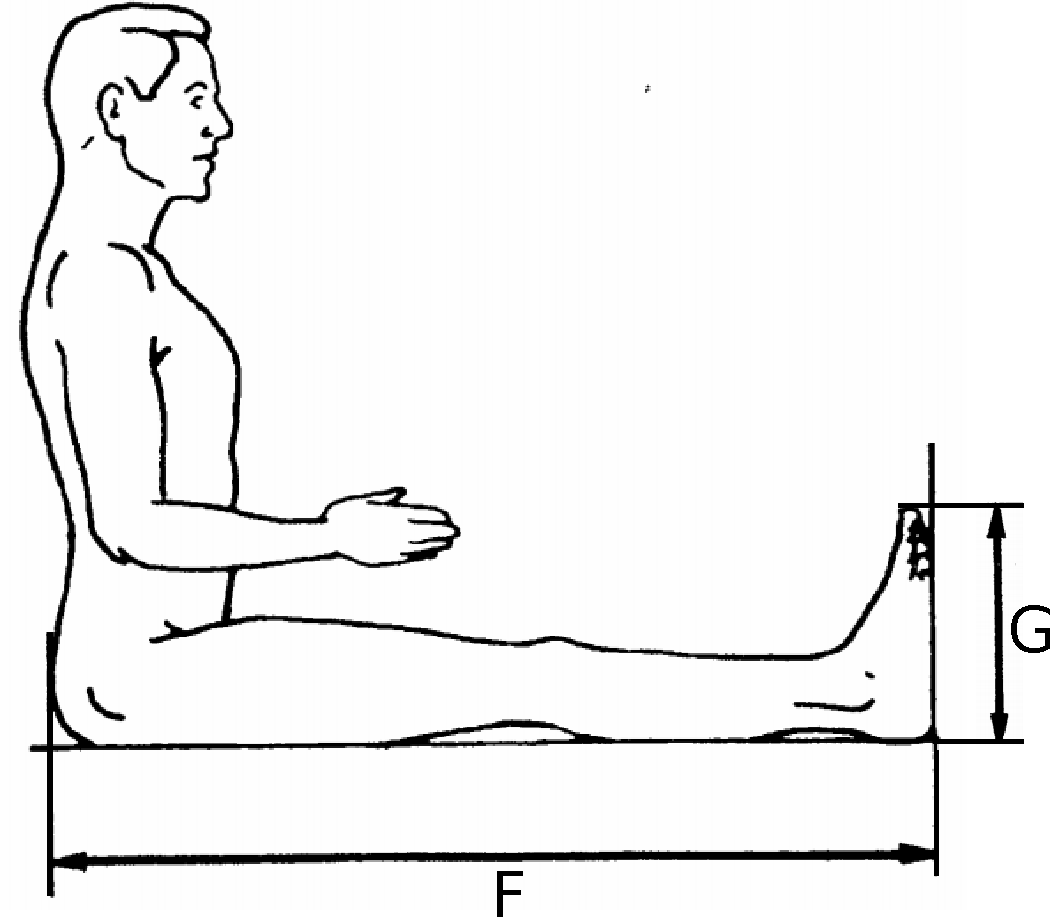
\includegraphics[width=\textwidth]{figures/din_measurements2.pdf}
        \caption{Hip}
        \label{fig:din2}
    \end{subfigure}
	\caption{Lower body measurements used for RuBi. Picture adapted from \cite{din_measurements1}.}
	\label{fig:human_measurements}
\end{figure}


\begin{table}
\begin{center}
	\begin{tabular}{c | c | c | c}
	  Index & Definition & Value & \% of Stature \\
	  \hline
	  A & Stature (body height) & ** & 100 \\
	  B & Crotch height & ** & ** \\
	  C & Femur height & ** & ** \\
	  D & Tibial height & Not in norm & **\\
	  E & Ankle-toe tip distance & Not in norm & ** \\
	  F & Buttocks-leg length & ** & ** \\
	  G & Sole length & ** & **
	\end{tabular}
	\caption{Human proportions from DIN 33402-2}
	\label{tab:din_proportions}
\end{center}
\end{table}

\subsection{Limbs length} % (fold)
\label{sub:limbs_lengths}
The dimensions needed to create a simplified model of one leg are the limbs lengths, which are the straight line distances measured from two consecutive joints.
They have been called $l_{i}$ where $i$ is the robot link + joint as per table \ref{tab:limb_index} and can be seen in Figure \ref{fig:kinematics}.
However, the norm does not determine all of them.

\begin{table}
\begin{center}
	\begin{tabular}{c | c | c}
	  $l_{i}$ & Limb \\
	  \hline
	  $l_{1}$ & Hip + thigh & C \\
	  $l_{2}$ & Knee + Foreleg & D\\
	  $l_{3}$ & Ankle + foot & E 
	\end{tabular}
	\caption{Limbs index}
	\label{tab:limb_index}
\end{center}
\end{table}

Since $C$ and $E$ are not standard measurements in industry, they have been obtained as follows:

\paragraph{The Femur height}
The crotch height, denoted as $B$ in the figure, has been averaged with the buttocks-leg length and the tibial height + an empirical approximation of the height of the ankle have been subtracted from the result, obtaining $C$.

\paragraph{The ankle-toe tip distance}
Since this distance is not standard either, it has been obtained once again adjusting the sole length with empirical measurements.
% subsection limbs_lengths (end)

\subsection{Hip and sole width} % (fold)
\label{sub:subsection_name}
The hip width sitting, as defined in the norm and for the same sample group than before, has been used as starting point to define the final width of the structure of the hip.
This standard measurement has been scaled down to a human of length L from hip joint to toe tip, which would correspond to $L=C+D+E$, using the proportion between stature and lower body lengths, also obtained from the norm.
The same process has been conducted to calculate the implemented width of the foot sole.

% subsection hip_sole_width (end)

No other standard measurement has been used as reference for the design, such as thigh or lower leg circumferences, since they do not affect the kinematics of the structure although they have a big influence in its dynamics.
The criteria followed to model the dynamics of the robot is explained in \ref{sec:physical_properties}.


%% Here we just describe the process followed to obtain the final dimensions. 
%% The final results are shown in Chapter Results --> add tables and Froude number calculus


% section dimensions (end)
%!TEX root = ../../../report.tex

\section{Inertial dimensions of the frame} % (fold)
\label{sec:physical_properties}
This section presents the theoretical guidelines followed during the design of RuBi regarding its dynamic model.
The calculations carried out are to be found in chapters \ref{cha:mathematical_model} and \ref{cha:design}. 
The determination of the geometrical dimensions for a robot model is in general a deterministic task in which all the parameters can be selected without dependencies or limitations.
However the inertial parameters of a robot will be the result of the selection of these dimensions, together with the materials utilized for the implementation and the configuration of the elements on the structure, among others.
Here, the goal of the adjustment of the final inertial parameters is not to mimic the dynamics of human legs as with the kinematics, but to reduce the power requirements for locomotion while ensuring robustness and reliability.
The main inertial parameters object of study here are the mass of the links, the positions of their CoM and their inertia moments.
Other parameters with an influence in the model dynamics such as friction forces or delays introduced by transmissions are not discussed here due to the complexity of its determination at this stage of the project.

\subsection{Mass of the links} % (fold)
\label{sub:mass_of_the_limbs}
The mass of each limb $i$ will depend on the materials used, their geometry and their density together with any other component added to the link (actuators, electronics, transmissions).
As explained before, keeping the overall mass of the frame as low as possible while guaranteeing the fulfillment of all the structural requirements, such as resistance and resilience, has been one of the main goals of the analyses conducted in the design of RuBi.
This criteria led to the allocation of the embedded electronics off the robot and aim at small electric actuators as the lightest possible solution for the actuation. 
The calculations to select the limb materials and profiles are to be found in \ref{sub:limb_profile}.
The final values of mass per limb have been obtained as an approximate sum of the components that constitute them, due to the complexity of measuring them directly or using system identification techniques. 
They can be seen in \ref{tab:limb_physical_properties} and they have been assumed to be concentrated in the CoM of each link for the computation of the dynamic model.

% subsection mass_of_the_limbs (end) 
\vfill
\subsection{Mass distributions} % (fold)
\label{sub:centers_of_mass}

\paragraph{Limbs center of mass} % (fold)
\label{par:limbs_center_of_mass}
The position of the center of mass (CoM) of each limb referred to its joint rotational axis is a function of its masses, their distributions and its geometry.
Their coordinates are given referred to a local reference frame attached to each joint, with its $Z$ axis perpendicular to the sagital plane and its $X$ and $Y$ axes parallel to its equivalents in the main reference frame in the hip, shown in Figure \ref{fig:kinematics}.
Its direct influence in the dynamics of the system is shown in \ref{sec_dynamic_model}, equation \ref{eq:N-E_eq1}.
The coordinates of the CoM of the limbs have been estimated during the design through the 3D CAD design software tool SolidWorks \cite{solidworks}.
Their final values can be found in \ref{tab:limb_physical_properties}.

% paragraph limbs_center_of_mass (end)

\paragraph{Center of mass of the frame} % (fold)
\label{par:center_of_mass_of_the_frame}
The location of the frame center of mass plays a very important role in the stability of the robot \cite{rojas}.
Its theoretical placement when standing still should be in the sagital plane of the structure, as close to the hip as possible, similar to humans (accounting that there is no torso).
A robust locomotion should result in a controlled and limited motion of the CoM. 
A high positioning of the CoM in the structure would make it more sensitive to the actuators influence, allowing a better balance control, while a lower placement in the structure could increase its robustness against inertial phenomenas.
The trade-off between these two criteria has been tried to be found.
As for the limbs, the coordinates of the CoM of the structure have been computed through SolidWorks and their final values can be found in %\ref{} reference to Results table and Implementation section

% paragraph center_of_mass_of_the_frame (end)

% subsection centers_of_mass (end)

\subsection{Moments of inertia} % (fold)
\label{sub:moments_of_inertia}
The inertia tensor of each limb will be the result of their distribution of masses with respect to the joint axis.
Since the kinematics analysis of the robot has been reduced to a planar case for both legs, as discussed in \ref{sec_kinematic_model}, the tensors have been reduced to a scalar value, their $I_{zz}$ component for the defined reference system.
The influence of the inertia moments of the limbs in the dynamics of the system can be seen in equation \ref{eq:N-E_eq1} where is, as per definition, the proportion between angular acceleration around the axis and torque applied.
This relationship yields another design criteria for the robot: the minimization of the inertia moments of the limbs in order to reduce the required torque applied for moving the limbs.
As for the previous magnitudes, the final inertia moments have been calculated with the CAD model in SolidWorks, and can be found in \ref{tab:limb_physical_properties}.
Their role in the simulation model developed in Gazebo is discussed in \ref{cha:simulation}. 

% subsection moments_of_inertia (end)

% section physical_properties (end)
%!TEX root = ../../../report.tex
\section{Joints design} % (fold)
\label{sec:joints}
Following the idea of mimicking the human lower-body structure it was decided to implement three actuated rotational joints per leg although some research was conducted on the use of passive ankles as in \cite{dacbot1}, \cite{phides} or \cite{mabel}.
However, the results introduced in \cite{grimmer} from their analysis of joint actuation for prosthetics limbs proved the importance of the actuation in the ankles for running.

The design of the joints entailed the addressing of three main areas:
\begin{itemize}
  \item Actuator model
  \item Transmission system
  \item Implementation of dedicated compliance
\end{itemize}

\subsection{Actuators} % (fold)
\label{sub:actuators}
In humans, the actuation of the joints is mostly provided by pairs of agonist-antagonist skeletal muscles linked to the bones through the tendons \cite{anatomy}.
The activation-inhibition of these muscles produce a lever effect on the bones that leads to its control and motion by modifying the angle between two consecutive limbs.
To achieve the same kind of motion control, the implementation of a similar system through electric linear actuators was considered.
However, the time constraints, their price and their complexity led to discard them and select conventional electric motors.
The selected motor model will have to be able to provide a sufficient torque to generate the desired forces at the end of the link, following equation \ref{eq:torque}.

\begin{equation}
\label{eq:torque}
  \tau = r \times F
\end{equation}

This equation could be sufficient to compute the torque required by the load for a motor application of leverage. 
However, a study of each joint separately would not provide an accurate enough solution due to the configuration of the legs, making necessary a study of the actuation as for a kinematic chain.
The analysis of the actuators requirements is to be found in \ref{cha:mathematical_model}.

% subsection actuators (end)

\subsection{Torque transmission} % (fold)
\label{sub:transmission}
As introduced in \ref{sub:moments_of_inertia}, the reduction of the moments of inertia in the limbs in order to minimize the torque requirements for motion was set as a priority.
This led to the study of methods to displace the CoM of the limbs as close to their joints axes as possible, thus reducing their inertias.
The solution was to place the actuators, the heaviest components of the design, as close to the upper part of the frame as possible, which would also result in the allocation of the CoM of the frame upper in the sagital plane.
An schematic example of this idea can be seen in the Figures in \ref{fig:compliance_series} for the ankle actuation, where the motor has been placed under the knee axis. 
The same principle has been applied to the knee actuation, as can be seen in the final implementation. 
For the hip, however, it was not necessary to install a transmission system, but a gear mechanism whose justification is to be found in \ref{cha:mathematical_model}.

Due to the new arrangement, a powertrain was required to transmit the torque to the joints.
It was decided to implement a system of 2 pulleys + belt due to its simplicity and optimal capabilities for the project requirements.
The goal of this mechanism is only the transmission of power, without any further adjustment of angular speed-torque ratios.
The calculations to find the optimal dimensions of the system are contained in \ref{sub:pulleys_and_belts}.
The pitfall of this implementation, however, is the introduction of delays in the motion transmission and the natural loss of accuracy arisen from the backlash associated to the use of pulleys.
Modeling these uncertainties for a classic locomotion controller based on the motion equations is proved a complex task. 
However it was assumed here that the ANN controllers that would drive the RuBi platform would be able to adapt to them without a model of the robot.

% subsection transmission (end)

\subsection{Joints compliance} % (fold)
\label{sub:compliance}
The advantages of the incorporation of compliance in legged locomotion have been broadly demonstrated in \cite{compliance_thesis} and \cite{grimmer}.
Compliance in running and walking gait generation is used to reduce actuators requirements through the minimization energy consumption.
Furthermore, it helps isolate the joints of the structure from the impact forces created during the landing phase, reinforcing the mechanical capabilities of the structure.
This section deals with the study and selection of the configuration of the elastic actuators and their distribution in the legs.
The numerical estimation of the actual springs to be used in the robot can be seen in \ref{sec_springs}.

\subsubsection{Elastic actuators configuration} % (fold)
\label{ssub:elastic_actuator_configuration}
Several elastic actuator configurations have been defined in the literature, from which four ones have been studied here and are shown in figures \ref{fig:pasive_actuators}.
The most detailed analysis of the influence of each of these configurations in energy storage and power consumption in human locomotion has been found in \cite{grimmer}.
In that paper, the normalized power requirements with the different configurations have been tested for a range of gaits, easing the process of finding the optimal configuration and its parameters for a specific gait and velocity.
However, the fact that RuBi is not being designed for a specific gait or velocity, but as a platform to study the transition between gaits and velocity adaption, makes the estimation of the best configuration an under-determined problem.
This reasoning led to the implementation of a new feature in RuBi, the full reconfigurability of the compliance in its actuators.
This capability allows for the possibility of studying in the real platform the influence of the elastic actuators on its performance and its control, giving RuBi a whole new set of uses.

\begin{figure}[h]
\centering
  \begin{subfigure}{.15\textwidth}
    %\centering
    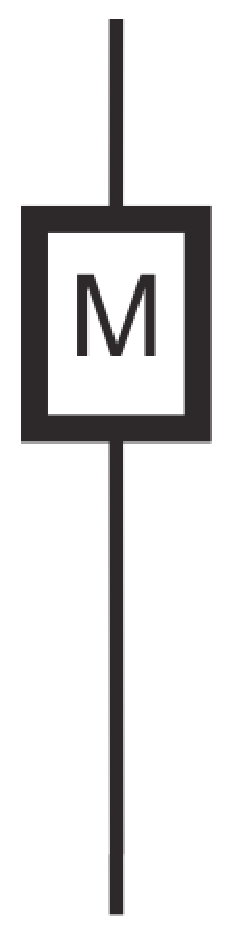
\includegraphics[width=0.63\linewidth]{figures/ddact.pdf}
    \caption{DD}
    \label{fig:dd}
  \end{subfigure}
  \begin{subfigure}{.15\textwidth}
    %\centering
    
\includegraphics[width=0.63\linewidth]{figures/SEAact.pdf}
    \caption{SEA}
    \label{fig:sea}
  \end{subfigure}
  \begin{subfigure}{.15\textwidth}
    %\centering
    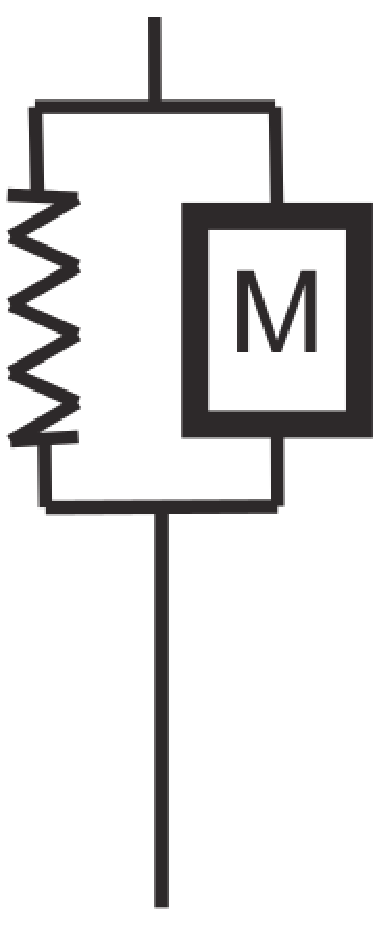
\includegraphics[width=\linewidth]{figures/PEAact.pdf}
    \caption{PEA}
    \label{fig:pea}
  \end{subfigure}
  \begin{subfigure}{.15\textwidth}
    %\centering
    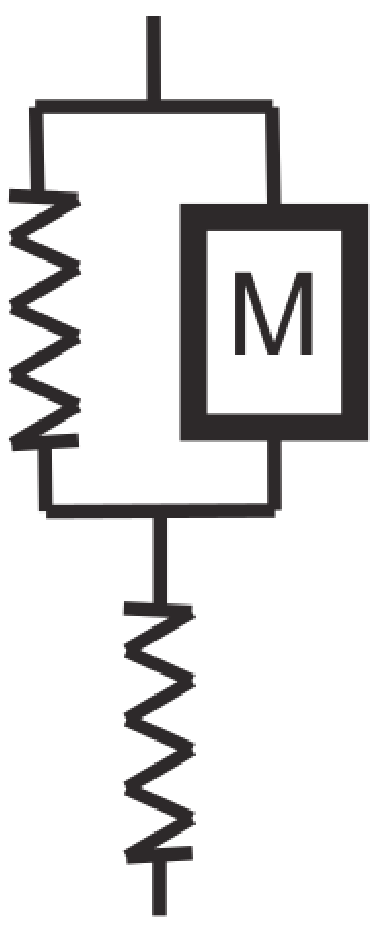
\includegraphics[width=\linewidth]{figures/SEA+PEAact.pdf}
    \caption{SEA+PEA}
    \label{fig:sea_pea}
  \end{subfigure}
  \caption{Four configurations for elastic actuators as from \cite{grimmer}}
  \label{fig:pasive_actuators}
\end{figure}  


%Flexible vs stiff drive train
%Power peak and average consumption comparisons --> energy storage 
%Protection against impact forces on landing phase
% subsubsection elastic_actuator_configuration (end)

\subsubsection{Compliance distribution and implementation} % (fold)
\label{ssub:compliance_distribution_and_possible_configurations}
The results in \cite{grimmer} demonstrate that the implementation of compliance in any of its variants in knees and ankles, influences notably the peak power and energy requirements both for walking and running.
They also seem to prove that the contribution to the reduction of energy consumption and power requirements of the hip is neglectable.
These findings have been used to justify the implementation of elastic actuators in knees and ankles, but not in the hip joints, actuated through direct transmission.

Several models from literature have been subject to a comparative analysis for their use in RuBi, being the main ones shown in Figure \ref{fig:compliance_series} and \ref{fig:compliance_parallel} for the ankle actuation (equivalent for the knees).
These schematics depict the three major design choices made so far, summarized in \ref{list:design_criterias}.
A short summary of the conclusions reached by these studies is introduced below.

\begin{itemize}
\label{list:design_criterias}
  \item Reduction of limbs inertias by placing the actuators up on the links.
  \item Use of transmission to solve the transfer of power motor-joint.
  \item Introduction of compliance through the use of springs.
\end{itemize}

\paragraph{SEA 1 and 2} % (fold)
\label{par:sea_1_2}
\ref{fig:series1} depicts an unidirectional SEA that has to be implemented together with a counterpart, which could be a passive spring or another actuator.
In that case the actuator task would only be the retraction of the foot to reduce its angle with respect to the lower leg, while the passive spring function would imitate the calf muscle.
This approach would be closer to the real functioning of the muscles in the legs, as explained in \ref{sec:bipedal_walking_and_running_gaits}.
However this configuration was discarded due to the complexity in the realization of a correct mapping between the angular displacement of the motor pulley and the ankle joint.

The configuration in Figure \ref{fig:series2} was found in \cite{biobiped}.
It solves the problem found for \ref{par:sea_1_2} changing the configuration of the motor and introducing a fixed pulley.
The influence of the relationship between $L_{B}$ and $L_{A}$ in the ratio between motor and joint torques was studies for this configuration in order to find the optimal dimensions.
However, this solution was discarded in favor of the current one, which demonstrated to be simpler to implement.
% paragraph sea_1_2 (end)

\begin{figure}[h]
\centering
  \begin{subfigure}{.19\textwidth}
    \centering
    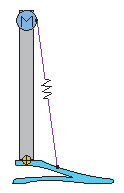
\includegraphics[width=\linewidth]{figures/illustration_serial_direct_i.pdf}
    \caption{SEA 1}
    \label{fig:series1}
  \end{subfigure}
  \begin{subfigure}{.2\textwidth}
    \centering
    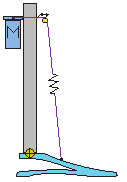
\includegraphics[width=\linewidth]{figures/illustration_serial_pulley.pdf}
    \caption{SEA 2}
    \label{fig:series2}
  \end{subfigure}
  \begin{subfigure}{.19\textwidth}
    \centering
    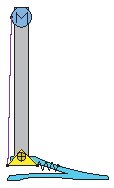
\includegraphics[width=\linewidth]{figures/illustration_serial_direct_ii.pdf}
    \caption{SEA 3}
    \label{fig:series3}
  \end{subfigure}
  \begin{subfigure}{.19\textwidth}
    \centering
    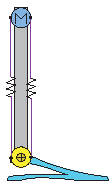
\includegraphics[width=\linewidth]{figures/illustration_serial_elastic_band.pdf}
    \caption{SEA 4}
    \label{fig:series4}
  \end{subfigure}
  \begin{subfigure}{.19\textwidth}
    \centering
    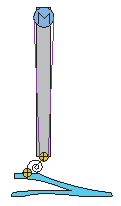
\includegraphics[width=\linewidth]{figures/illustration_serial_rotational.pdf}
    \caption{SEA 5}
    \label{fig:series5}
  \end{subfigure}
  \caption{SEA configurations studied}
  \label{fig:compliance_series}
\end{figure}  

\paragraph{SEA 3} % (fold)
\label{par:sea_3}
The spring configuration in \ref{fig:series3} was found in \cite{grimmer} for a prosthetic ankle design (meaning that the configuration should be adapted for the knee).
It was just used as a study case and source of ideas. 
% paragraph sea_3 (end)

\paragraph{SEA 4} % (fold)
\label{par:sea_4}
The configuration in \ref{fig:series4} was also found in \cite{biobiped} and is known as bidirectional SEA.
It was considered the most optimal to mimic the human musculature on the legs and its implementation through springs attached to the belts or with elastic bands (bungee cords) like the utilized in \cite{imperial_college} was object of analysis.
% paragraph sea_4 (end)

\paragraph{SEA 5} % (fold)
\label{par:sea_5}
The configuration called SEA 5 and shown in Figure \ref{fig:series5} was the selected one.
The original idea was taken from \cite{phides} but has been modified to ease its construction and provide more robustness to the final design.
In \cite{phides} this elastic transmission is implemented with torsion bars for the joints axes, while RuBi uses torsion springs placed around more resistant axis to transmit the motion.
% paragraph sea_5 (end)

\begin{figure}[ht!]
\label{fig:compliance_parallel}
\centering
  \begin{subfigure}{.19\textwidth}
    \centering
    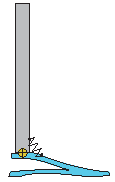
\includegraphics[width=\linewidth]{figures/illustration_parallel_prismatic.pdf}
    \caption{PEA 1}
    \label{fig:parallel1}
  \end{subfigure}
  \begin{subfigure}{.19\textwidth}
    \centering
    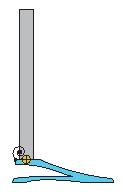
\includegraphics[width=\linewidth]{figures/illustration_parallel_rotational.pdf}
    \caption{PEA 2}
    \label{fig:parallel2}
  \end{subfigure}
  \caption{PEA configurations studied}
\end{figure}  

\paragraph{PEA 1} % (fold)
\label{par:pea_1}
The configuration in \ref{fig:parallel1} shows a compression spring (or extension spring depending the placement) connected within the two links.
This direct connection act as a parallel spring and has the advantage of being a very flexible system in terms of changing the physical parameters of the spring. 
However its design was discarded in favor of the rotational due to the previous election of the rotational series spring.
% paragraph pea_1 (end)

\paragraph{PEA 2} % (fold)
\label{par:pea_2}
The configuration called PEA 2 and shown in Figure \ref{fig:parallel2} was the selected one.
This is congruent with the series spring what will facilitate its integration when designing.
It also has the advantage of having common interfaces which would lead to the possibility of using the same springs for series and parallel configurations, saving thus money and time.

% paragraph pea_2 (end)


% Based on the experiments carried out in \cite{grimmer}, can be deduced that both PEA and SEA configurations have the advantages of reduce the peak and energy requirements of the motors.
% This causes a general improvement of the system due to if smaller motors are needed, the robot will be lighter and thus the structure of the link will weight less too.
% When comparing both configurations though, it is not exactly clear what are the benefices and the pitfalls of SEA, PEA and SEA+PEA.
% This is why a system that allows to have all the configurations is decided which would let the user to choose and implement its own configurations (SEA, PEA or SEA+PEA) and study their behaviors along with the controllers.
\todo{a paragraph has been commented. check if useful or not. i dont think so}
% subsubsection compliance_distribution_and_possible_configurations (end)

% subsection compliance (end)

% section joints (end)

% chapter analysis (end)